\documentclass{acmart}   
\usepackage[utf8]{inputenc} 
\usepackage[greek , english]{babel}
\usepackage{alphabeta}
\usepackage{hyperref} 
\usepackage{listings}
\usepackage{color}
\usepackage{float}
% \addbibresource{bibl.bib}
\usepackage[]{graphicx}
\graphicspath{{images/}}
\definecolor{mygreen}{rgb}{0,0.6,0}
\definecolor{mygray}{rgb}{0.5,0.5,0.5}
\definecolor{mymauve}{rgb}{0.58,0,0.82}

\begin{document}
       \begin{titlepage}
              \begin{center}
              \vspace*{1.5cm}

              \line(1,0){\textwidth}\\
              \textbf{Πρότζεκτ Προγραμματισμού Διαδικτύου}\\
              \vspace{0.2cm}
              Τμήμα Ηλεκτρολόγων Μηχανικών \& Τεχνολογίας Υπολογιστών\\
              \line(1,0){\textwidth}\\
               
              \vspace{1.5cm}
              
              \textbf{
              ΕΦΑΡΜΟΓΗ ΑΝΑΖΗΤΗΣΗΣ ΑΚΙΝΗΤΩΝ\\
              Ομάδα 3\\} 
              \vspace{1cm}

              \textbf{Αλκίνοος-Νικόλας Αλυσσανδράκης}\\
              Κατεύθυνση: Υπολογιστές\\
              ΑΜ: 1234567<----\\
              Έτος Φοίτησης: 4ο\\
              \vspace{0.8cm}
              \textbf{Δήμητρα-Μαρία Σκαμαντζούρα}\\
              Κατεύθυνση: Τεχνολογία της πληροφορίας\\
              ΑΜ: 1072713\\
              Έτος Φοίτησης: 4ο\\

              \vspace{0.8cm}

              % \includegraphics[width=0.4\textwidth]{university}

              
              \end{center}
       \end{titlepage}
\tableofcontents
\newpage

\section{Περίληψη}
Το θέμα του πρότζεκτ που ανατέθηκε στην ομάδα μας είναι η υλοποίηση μίας ιστοσελίδας αναζήτησης ακινήτων. Τα ακίνητα αυτά εμφανίζονται σε μορφή αγγελιών, όπου οποιοσδήποτε μπορεί να έχει πρόσβαση και να αζητήσει με βάση τις επιθυμίες του. Στους χρήστες δίνεται η επιλογή δημιουργίας λογαριασμού, η οποία παρέχει τα προνόμια της προσθήκης αγγελιών στα αγαπημένα και την συγκρώτηση τους σε μία λίστα αγαπημένων στο προφίλ του χρήστη. Στις αγγελίες παρουσιάζονται τα στοιχεία του αγγελιοδότη και ο χρήστης μπορεί να έρθει σε επικοινωνία με τον αγγελιοδότη, εφόσον το επιθυμεί.

\section{Μεθοδολογια}
\subsection{Στόχος}
Ο κύριος στόχος, κατά την υλοποίηση του πρότζεκτ, ήταν η πραγματοποίηση της κύριας αναζήτησης. Βασικά χαρακτηριστικά αυτής αποτελούσαν η περιοχή, το είδος ακινήτου, το εύρος της τιμής και του εμβαδού, καθώς επίσης το είδος της αγγελίας. Σε επόμενο στάδιο, επιθυμητό ήταν να προβάλλονταν στον χρήστη όλες οι αγγελίες ακινήτων που πληρούσαν τις προϋποθέσεις με όλες τις βασικές τους πληροφορίες.

\subsection{Υλοποίηση}
\subsection*{Προσέγγιση}
Πρώτο βήμα μετά την ανάθεση του θέματος ήταν να αναζητήσουμε αντίστοιχα παραδείγματα ιστοσελίδων και να κρίνουμε ποια χαρακτηριστικά θεωρούσαμε απαραίτητα για την ιστοσελίδα. Σε συνέχεια, υλοποιήσαμε το UI/UX design της εφαρμογής με χρήση του figma και κανονίσαμε μία συνάντηση με τον κ. Αβούρη, προκειμένου να εκφέρει την αποψή του και να έχουμε το απαραίτητο feedback. Έχοντας αποκτήσει μία ξεκάθαρη εικόνα του περιεχομένου της ιστοσελίδας, προχωρήσαμε στον διαμοιρασμό της δουλειάς. Ο ένας ασχολήθηκε κατα κύριο λόγο με το front-end (Σκαμανατζούρα Δήμητρα) και ο άλλος με το back-end (Αλκίνοος Αλυσσανδράκης).

\subsection*{Εργαλεία και Τεχνολογίες}
Για την δημιουργία του front end τομέα της ιστοσελίδας αξιοποιήθηκαν οι εξής τεχνολογίες:
\begin{itemize}
       \item Handlebars
       \item CSS3
       \item Javascript
\end{itemize}
To handlebars εξηπυρετούσε τον σκοπό της ύπαρξης templates και την δυναμική δημιουργία των html που απευθύνονταν στον χρήστη.\\
Αντίστοιχα για το κομμάτι του back end:
\begin{itemize}
       \item Node.js
       \item Express
       \item mongodb <------
       \item Javascript
\end{itemize}

\subsection*{Χρονοδιάγραμμα}
Τα βήματα που πάρθηκαν χρονικά ήταν ως εξής:
\begin{itemize}
    \item Ορισμός των βασικών χαρακτησριστικών της σελίδας
    \item Σχεδιασμός σελίδας στο χαρτί
    \item Σχεδιασμός σε figma
    \item Υλοποίηση σελίδων με χρήση html και css
    \item Backend<------
\end{itemize}

\subsection*{Δημιουργια ERD και βασης δεδομένων}

------>
 
\subsection{Front-end}
Αρχικά, σε κάθε σελίδα υπάρχουν δύο βασικά στοιχεία, το λογότυπο της ιστοσελίδας μας και το εικονίδιο σύνδεσης χρήστη. Αν ο χρήστης κάνει κλικ πάνω στο εικονίδιο με το λογότυπο, τότε θα γίνει παραπομπή στην αρχική σελίδα, αν κάνει κλικ στο εικονίδιο χρήστη τότε θα εμφανιστεί το αντίστοιχο pop-up, αναλόγως αν είναι συνδεδεμένος ή όχι ο χρήστης. Η μορφή αυτών των pop-ups παρουσιάζεται στην εικόνα \emph{Fig. 1}.
\begin{figure}[H]
       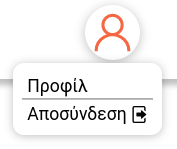
\includegraphics[width=0.2\textwidth]{pop-up_1.png}
       
\includegraphics[width=0.15\textwidth]{pop-up_2.png}
       \caption{Pop-ups}
       \label{fig:pop-ups}
\end{figure}
\subsection*{Αρχική Σελίδα}
Η πρώτη υλοποίηση, από άποψης front-end, ήταν η αρχική σελίδα της ιστοσελίδας. Έμπνευση για την συνολική εικόνα της ιστοσελίδας αποτέλεσαι κατά κύριο λόγo η σελίδα του σπιτόγατου (\href{www.spitogatos.gr}{Spitogatos}). 
Σε συνέχεια, βασική λογική της αρχικής σελίδας αποτελεί η επιλογή ενός εκ των δύο πιθανόν σεναρίων, ενοικίασης ή πώλησης. Επιπλέον, πριν ο χρήστης προχωρήσει στην αναζήτηση, μπορεί να συμπληρώσει παραπάνω χαρακτηριστικά, όπως η περιοχή, η κατηγορία του ακινήτου κτλ.
\begin{figure}[H]
       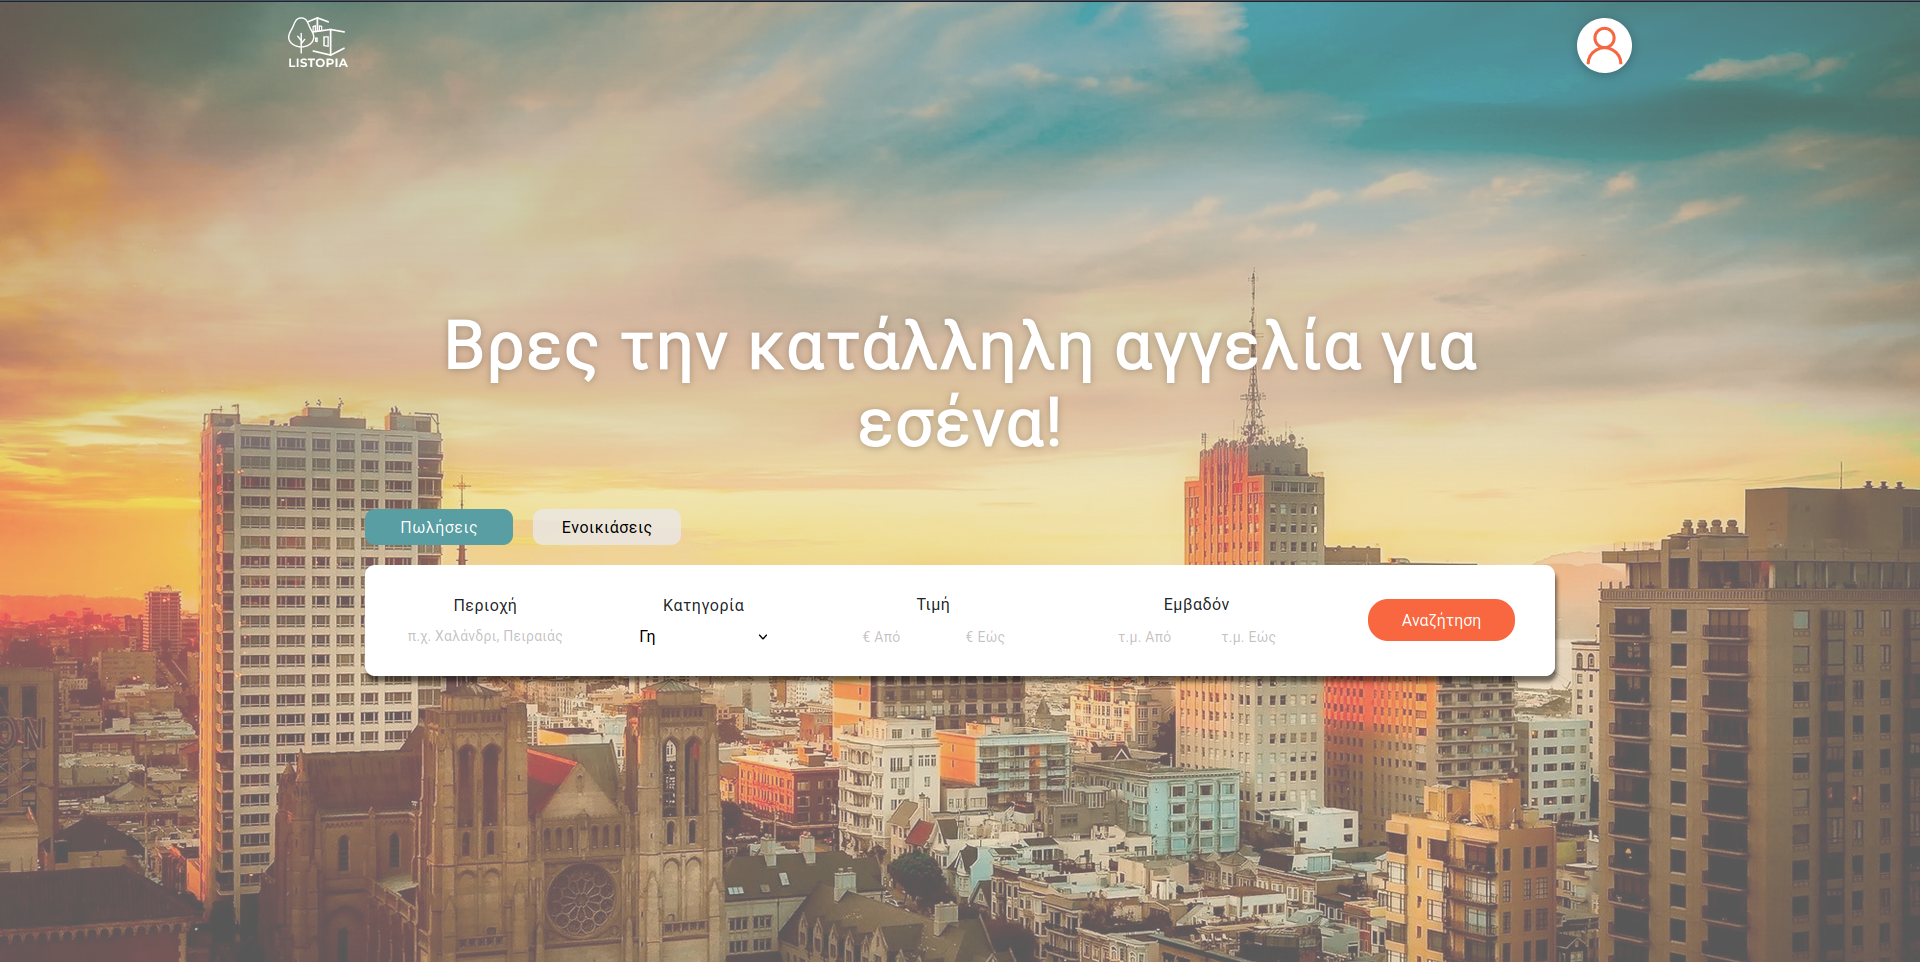
\includegraphics[width=0.8\textwidth]{home_page.png}
       \caption{Αρχική Σελίδα}
       \label{fig:home}
\end{figure}
\subsection*{Σελίδα Αποτελέσματα Αναζήτησης}
Στην συνέχεια, η σελίδα προβολής των αποτελεσμάτων αναζήτησης είναι αναγκαία για την λειτουργικότητα της. Βασικό στοιχείο της υλοποίησης αποτελεί η προβολή των καρτών των αγγελιών που πληρούν τα χαρακτηριστικά που έχει δηλώσει ο χρήστης. Αυτές οι κάρτες αποτελούνται από μία εικόνα του ακινήτου, τα βασικά χαρακτηριστικά της αγγελίας, όπως τύπος, εμβαδόν, τιμή κλπ. Εφόσον ο χρήστης πατήσει κάποια από αυτές τις κάρτες, θα μεταφερθεί στην αντίστοιχη σελίδα της συγκεκριμένης αγγελίας. Επιπλέον, σε κάθε κάρτα υπάρχει η επιλογή τοποθέτησης της συγκεκριμένης αγγελίας στα αγαπημένα μέσω της καρδούλας που εμφανίζεται στην κάρτα.
Έπειτα, λοιπά χαρακτηριστικά αυτής της σελίδας είναι η επιστροφή πίσω στην αρχική αλλά και η επιλογή φίλτρων αναζήτησης. Η μπάρα με τα φίλτρα εμφανίζεται πατώντας πάνω στο κουμπί που αναγράφει "Φίλτρα" και ξανακλείνει με τον ίδιο ακριβώς τρόπο.
\begin{figure}[H]
       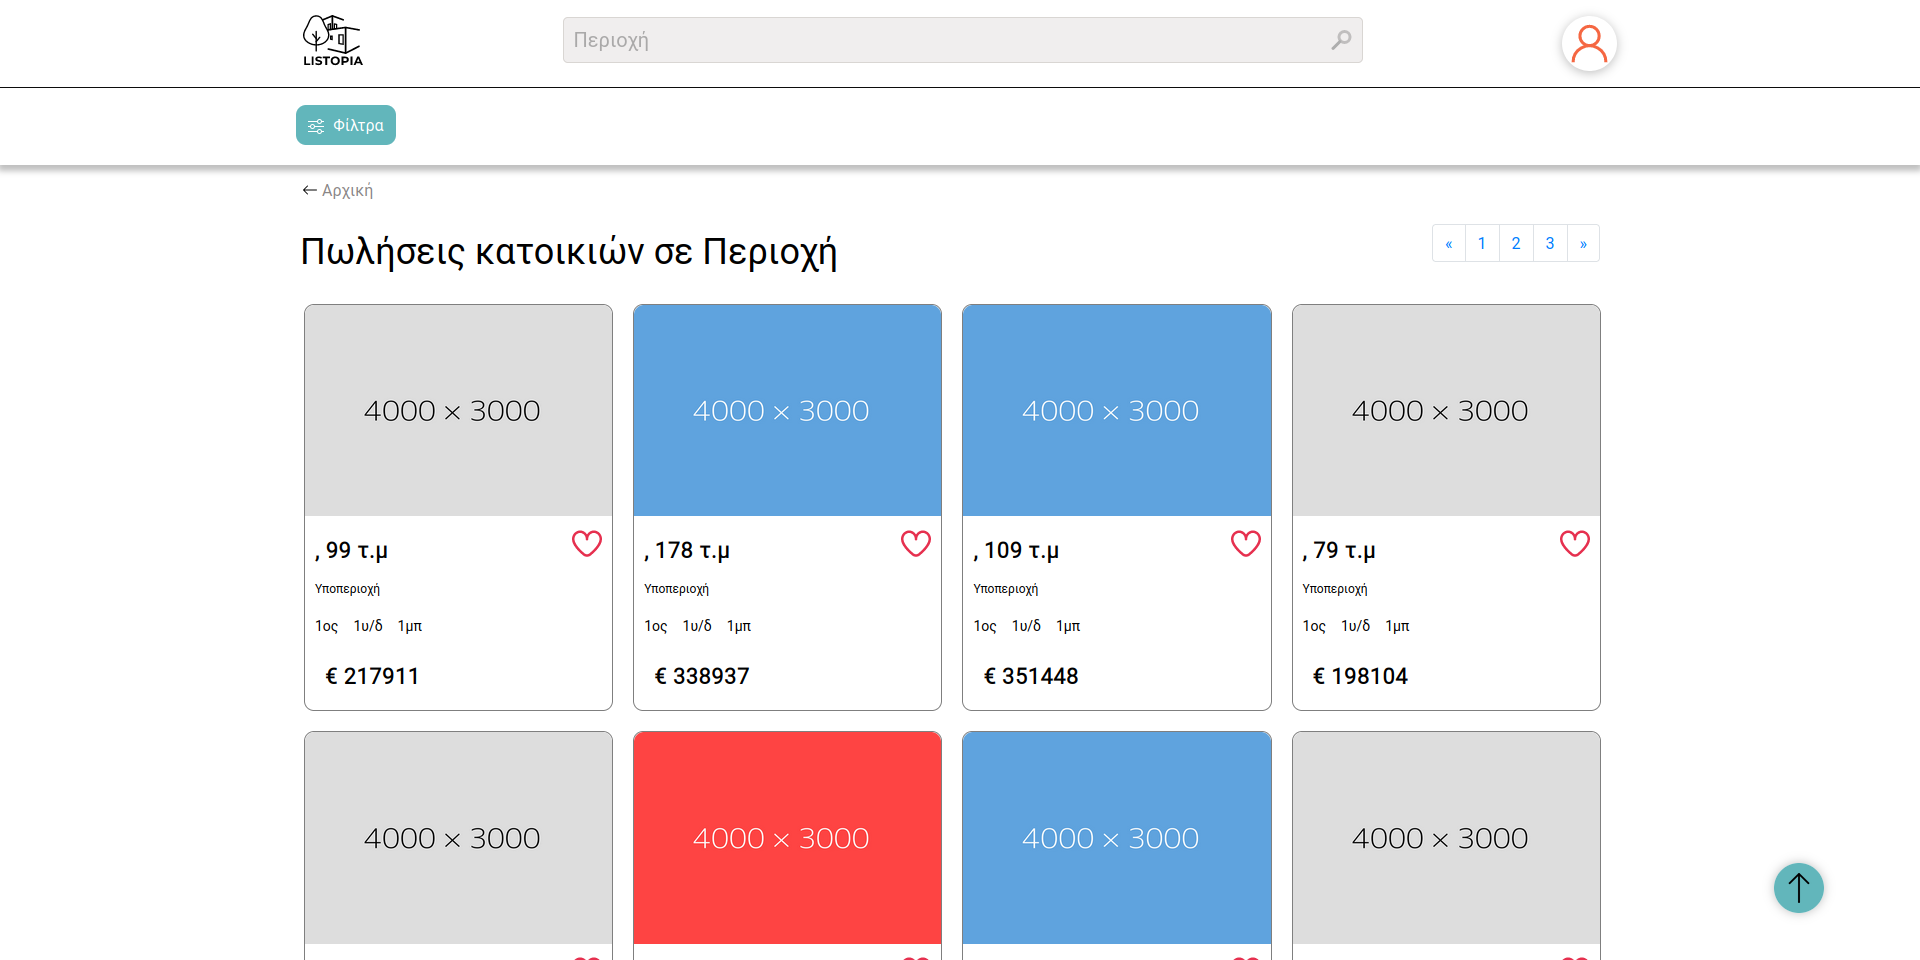
\includegraphics[width=0.8\textwidth]{search_page.png}
       \caption{Αποτέλεσμα Αναζήτησης}
       \label{fig:events}
\end{figure}
\begin{figure}[H]
       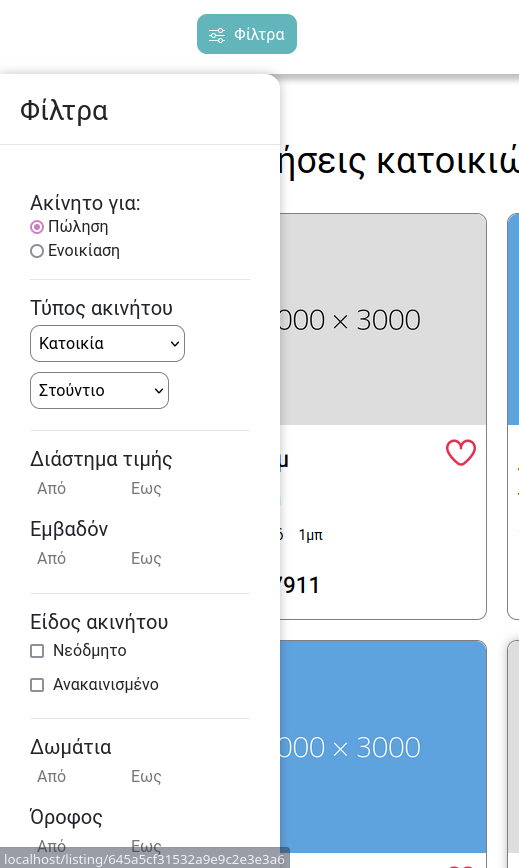
\includegraphics[width=0.5\textwidth]{filter.png}
       \caption{Φίλτρα}
       \label{fig:edit}
\end{figure}
\subsection*{Σελίδα Αγγελίας}
Κύριο χαρακτηριστικό της σελίδας αυτής αποτελεί ο τομέας των εικόνων. Οι εικόνες εμφανίζονται με την δομή που παρουσιάζεται στην εικόνα \emph{Fig. 5} και σε περίπτωση που ο χρήστης πατήσει πάνω τους ανοίγει ένα pop-up carousel. Σε αυτό, ο χρήστης μπορεί να πλοηγήσει όλες τις διαθέσιμες εικόνες αυτού του ακινήτου όπως παρουσιάζεται στην εικόνα \emph{Fig. 7}.
Επιστρέφοντας στην αρχική όψη αυτής της σελίδας, ο χρήστης κάνοντας σκρολ προς τα κάτω μπορεί να ενημερωθεί για όλες τις λοιπές πληροφορίες για το συγκεκριμένο ακίνητο. Σε περίπτωση που ενδιαφέρεται, παρουσιάζονται τα στοιχεία επικοινωνίας του αγγελιοδότη και έτσι μπορεί να έρθει σε επικοινωνία μαζί του.
\begin{figure}[H]
       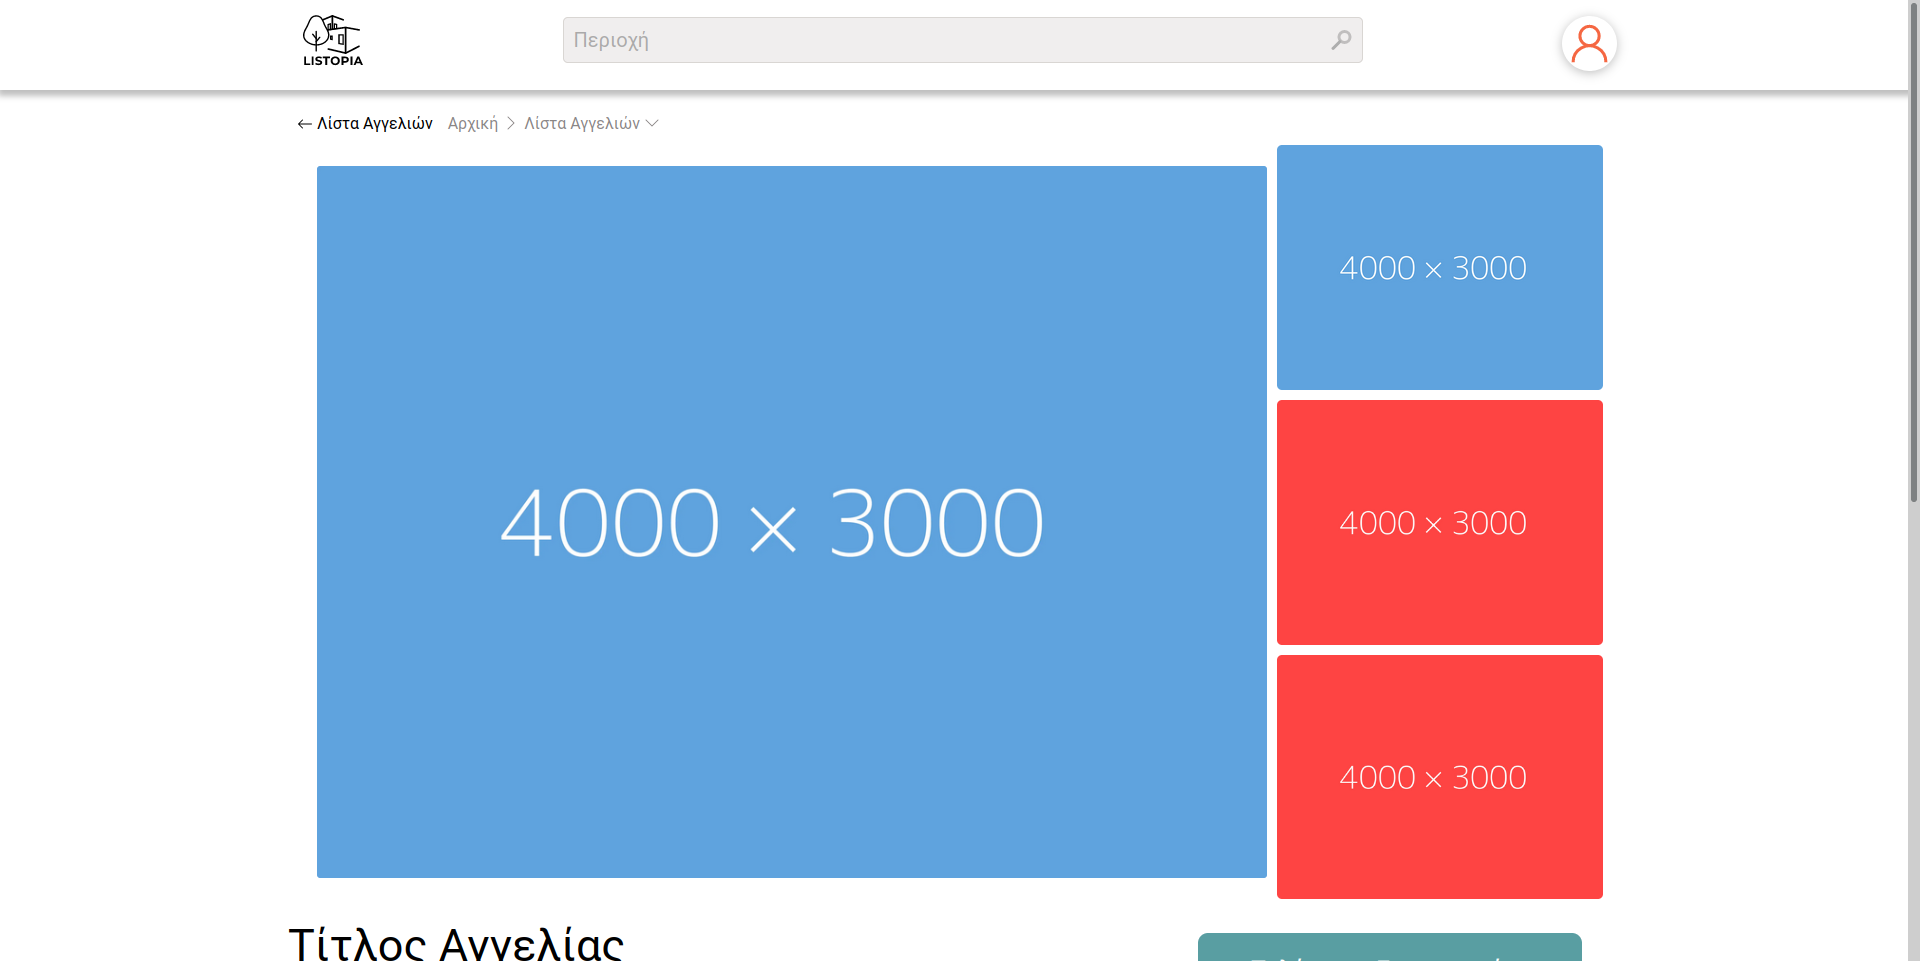
\includegraphics[width=\textwidth]{listing_page1.png}
       \caption{Αγγελία Κομμάτι 1}
       \label{fig:event}
\end{figure}
\begin{figure}[H]
       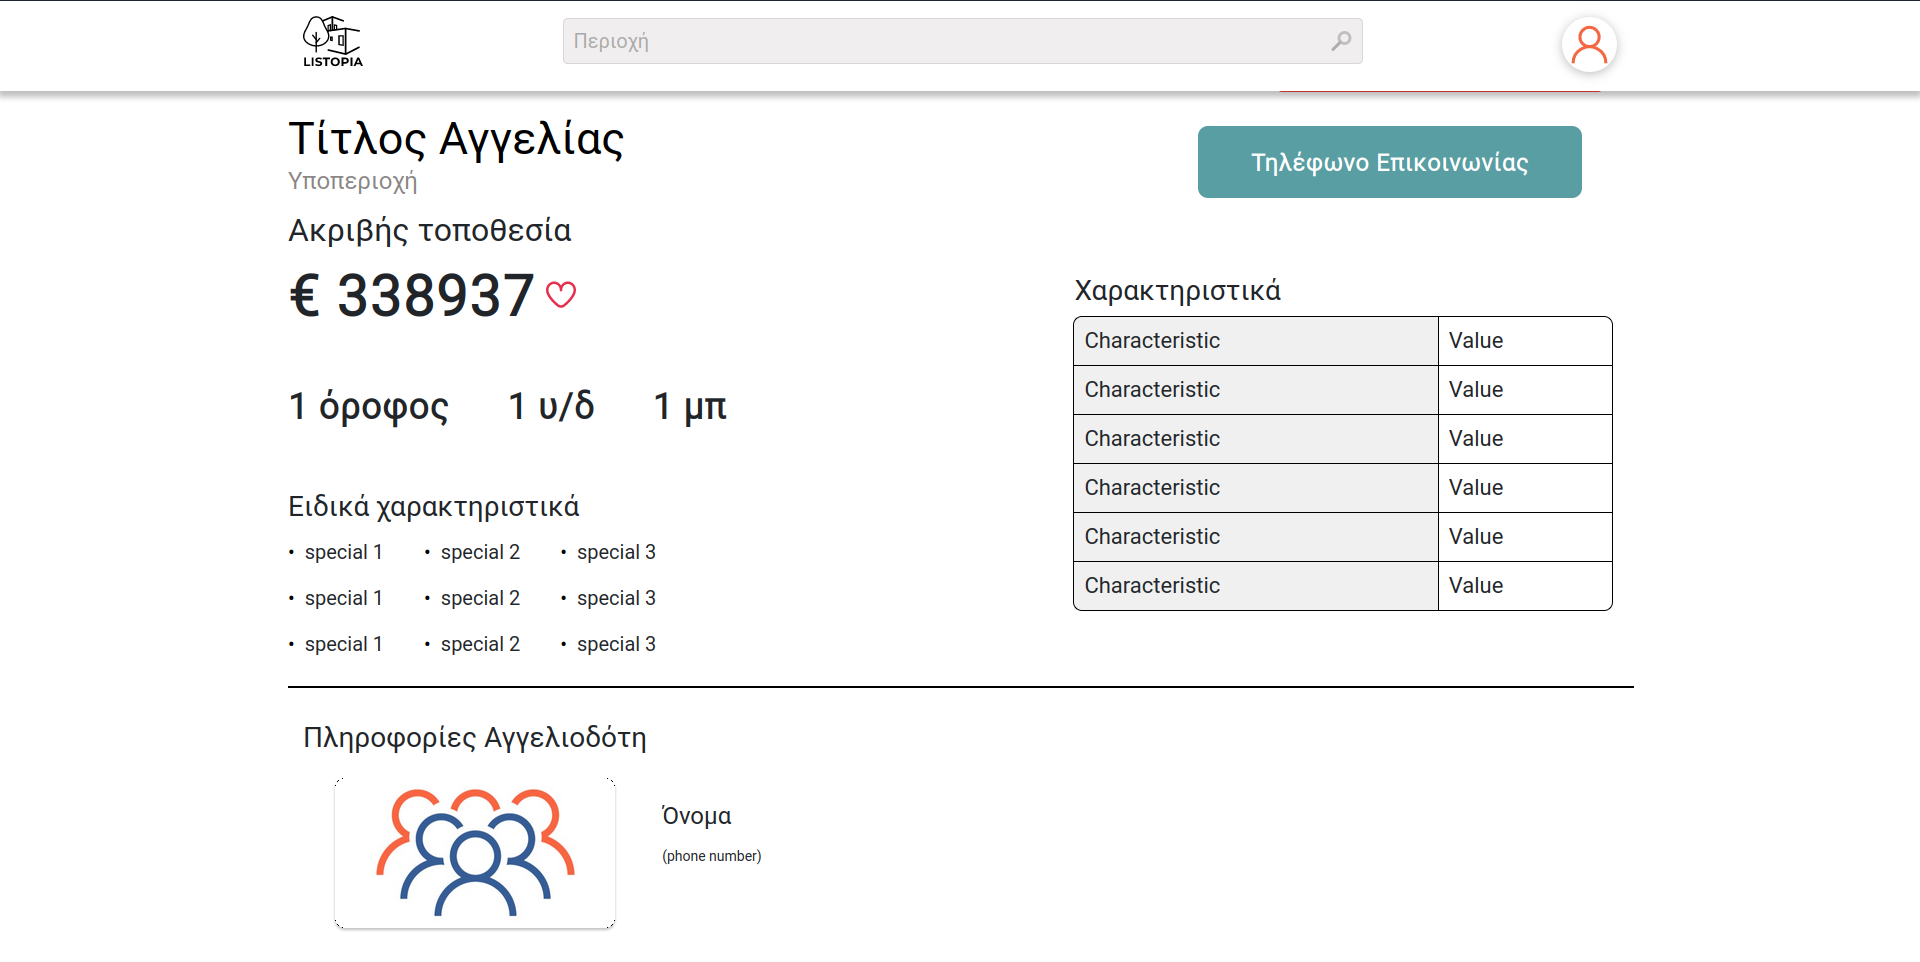
\includegraphics[width=\textwidth]{listing_page2.png}
       \caption{Αγγελία Κομμάτι 2}
       \label{fig:event}
\end{figure}
\begin{figure}[H]
       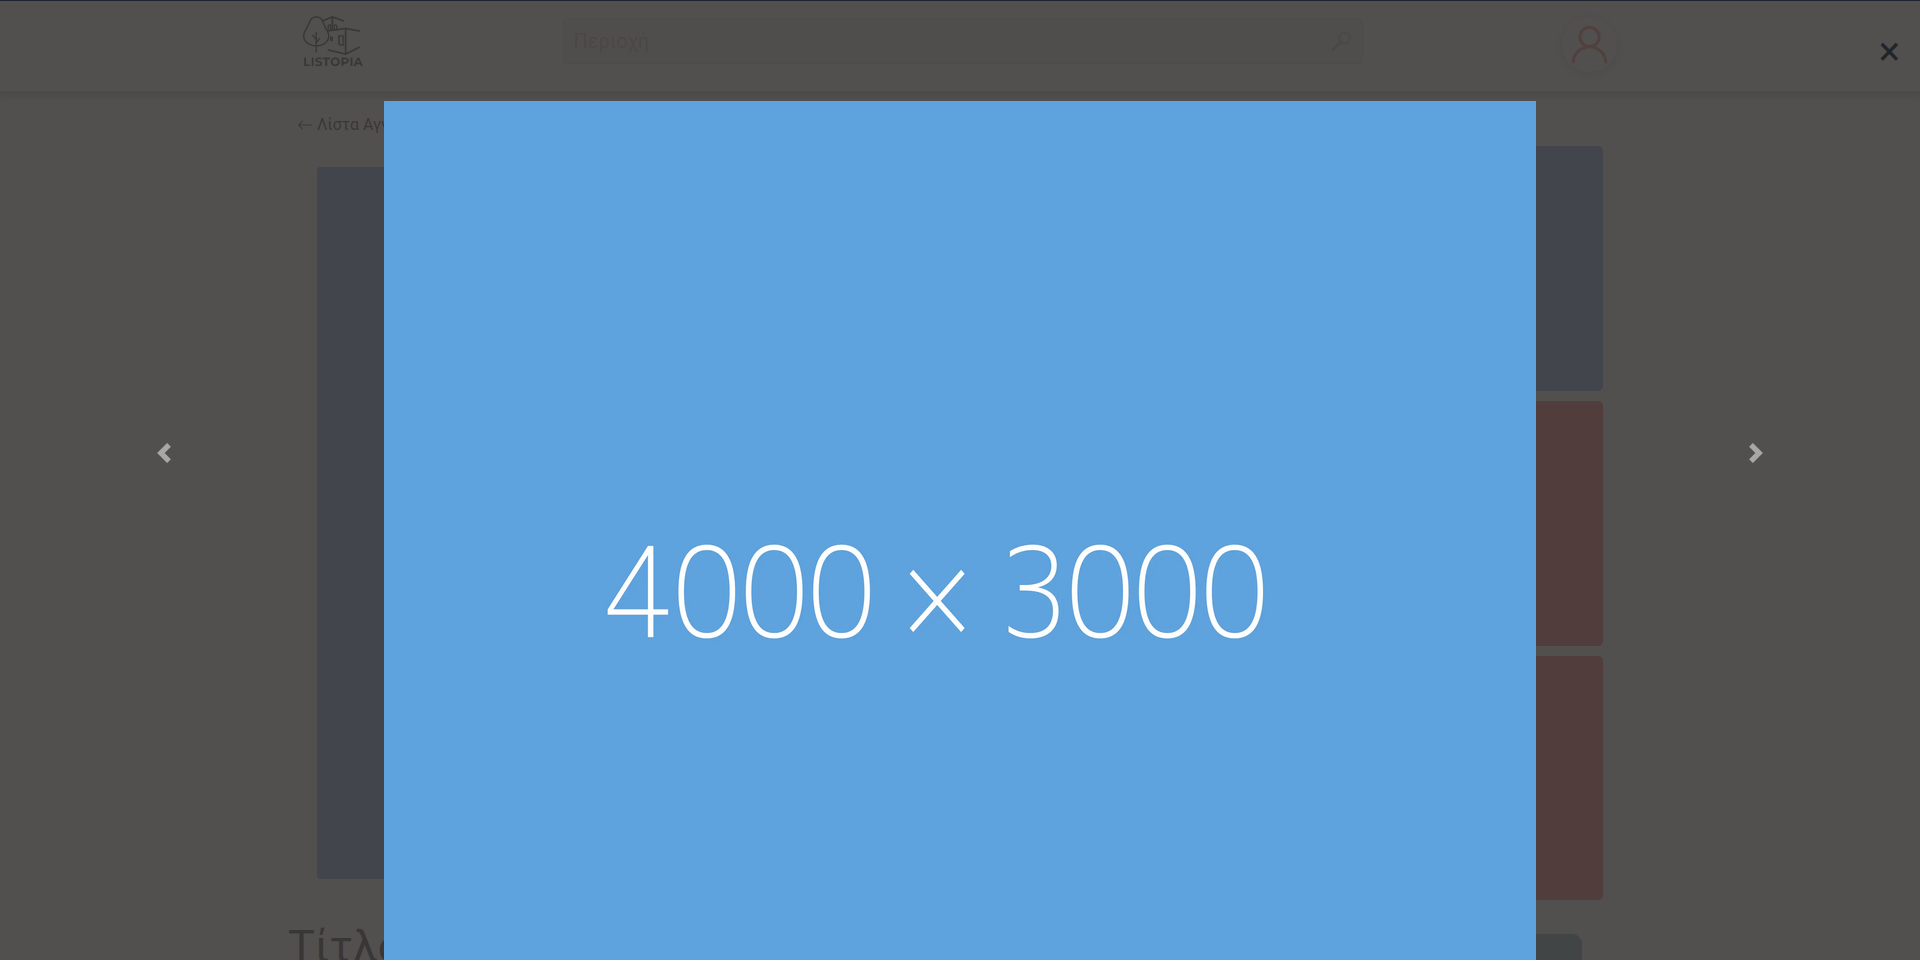
\includegraphics[width=0.8\textwidth]{listing_carousel.png}
       \caption{Carousel Φωτογραφιών}
       \label{fig:event}
\end{figure}
\subsection*{Σελίδες Εισόδου και Εγγραφής}
Όσο αφορά την δημιουργία λογαριασμού στην εφαρμογή, ζητείται από τον χρήστη να συμπληρώσει κάποια απαραίτητα χαρακτηριστικά όπως μία διεύθυνση ηλεκτρονικού ταχυδρομίου, το όνομα του και τέλος τον κωδικό του όπως φαίνεται στην εικόνα \emph{Fig. 9}. Εφόσον γίνουν όλα αυτα επιτυχώς, είναι εφικτή η σύνδεση του στην σελίδα. Για την σύνδεση του, ζητείται η συμπλήρωση της διεύθυνσης ηλεκτρονικού ταχυδρομίου και κωδικός που υπέβαλλε κατά την εγγραφή του όπως φαίνεται και στην εικόνα \emph{Fig. 8}.
\begin{figure}[H]
       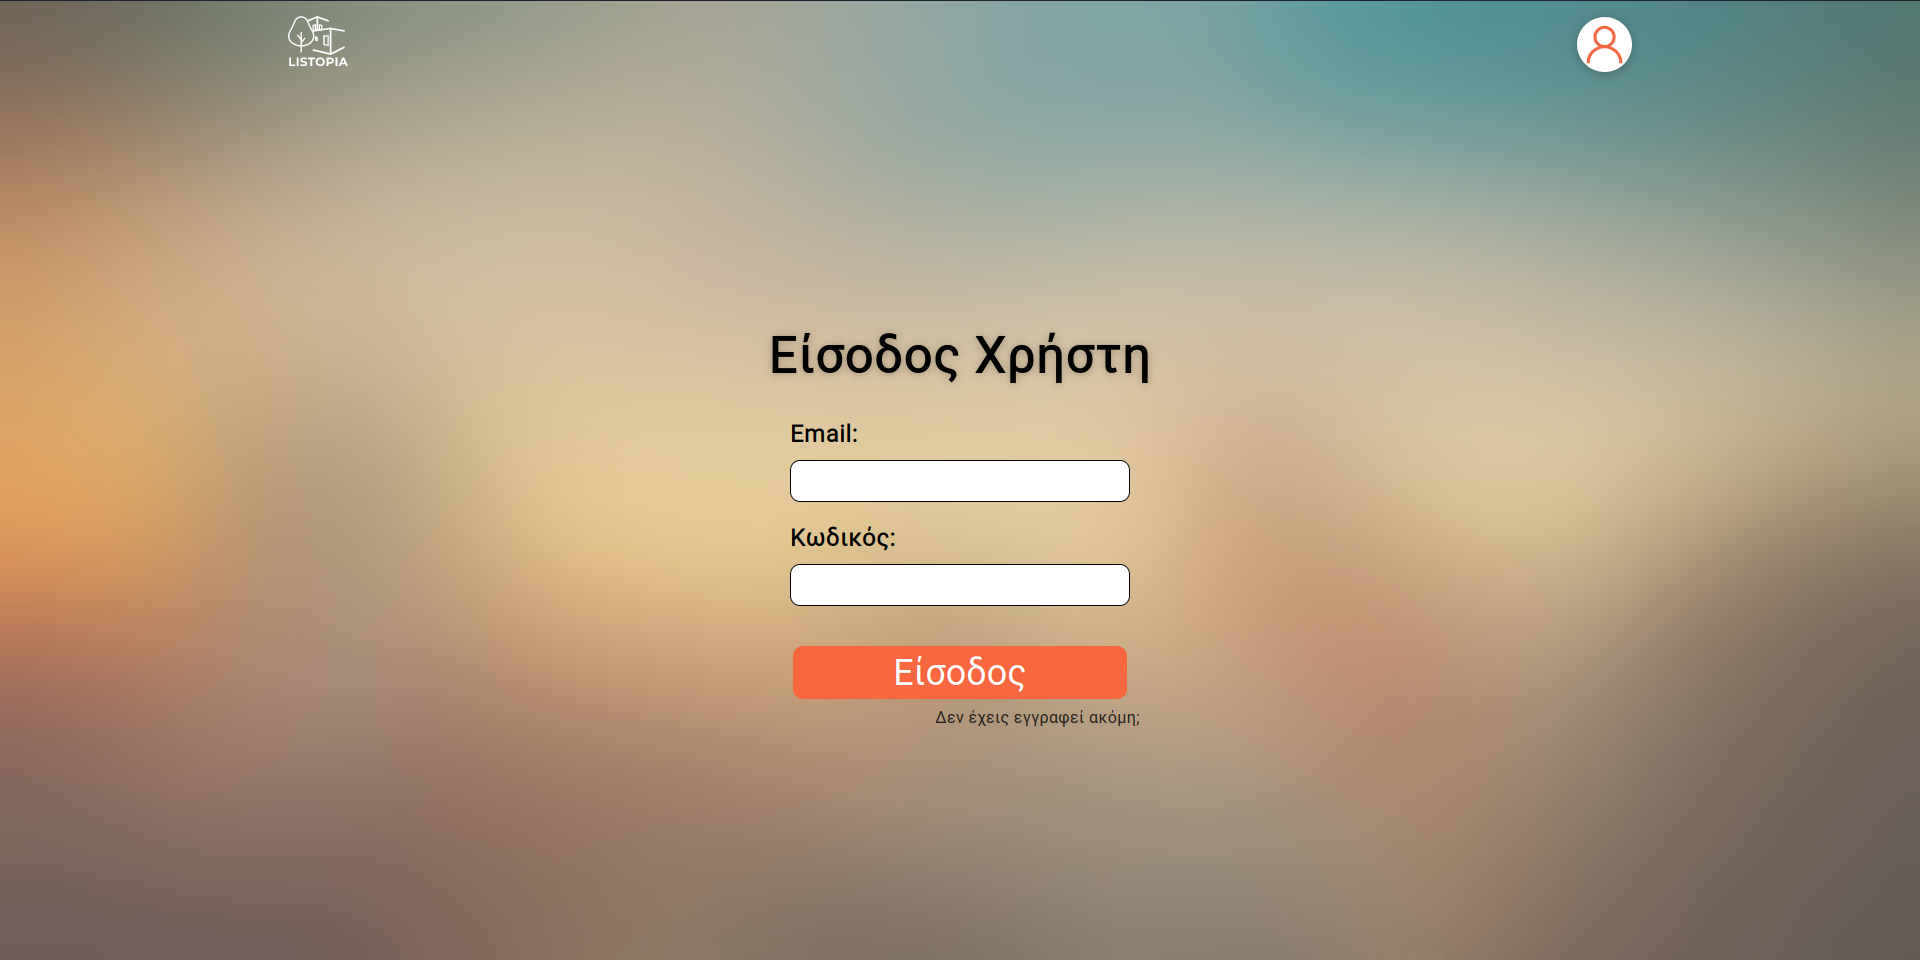
\includegraphics[width=0.8\textwidth]{sign_in_page.png}
       \caption{Είσοδος Χρήστη}
       \label{fig:reserve}
\end{figure}
\begin{figure}[H]
       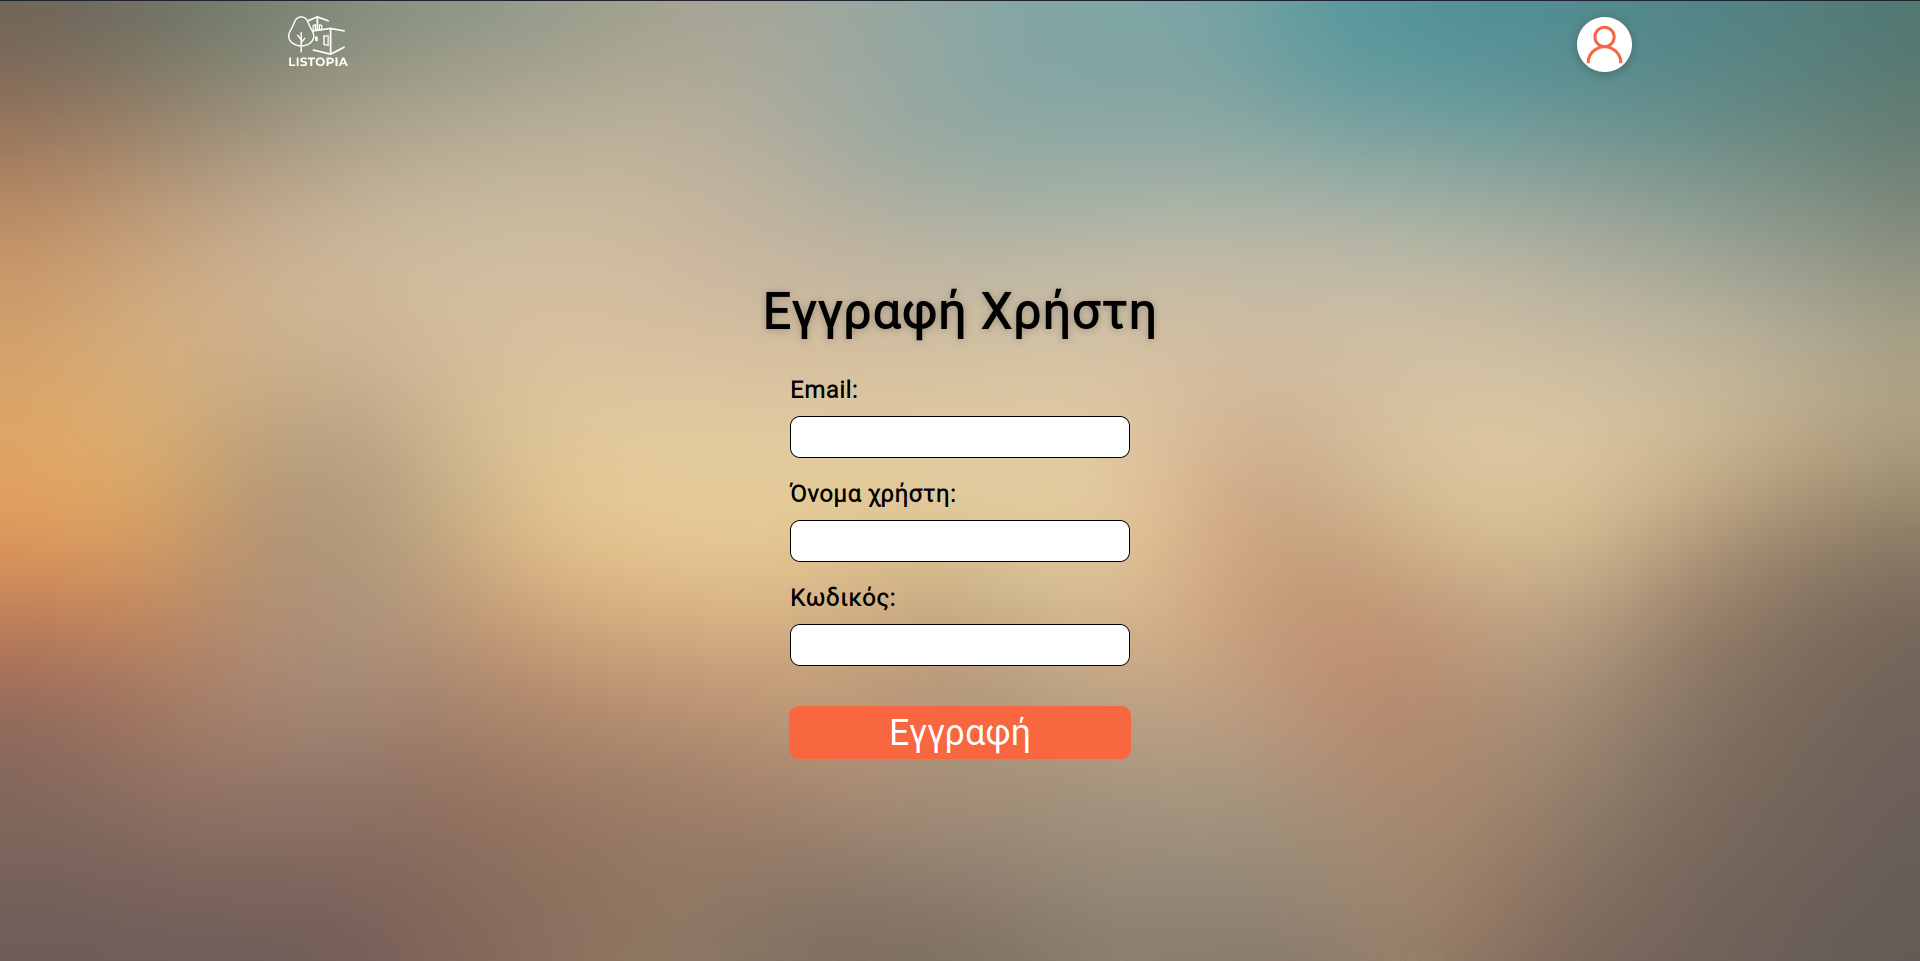
\includegraphics[width=0.8\textwidth]{sign_up_page.png}
       \caption{Εγγραφή Χρήστη}
       \label{fig:about}
\end{figure}
\subsection*{Σελίδα Προφίλ Χρήστη}
Εφόσον ο χρήστης έχει συνδεθεί, στην σελίδα του Προφίλ του παρουσιάζονται τα στοιχεία που έχει συμπλήρώσει και του δίνεται η επιλογή να τα τροποποιήσει και να τα αποθηκεύσει. Επιπλέον, παρουσιάζονται σε μία λίστα αγαπημένων όλες οι αγγελίες που έχει προχωρήσει στην καταχωρησή τους ως αγαπημένα, εφόσον υπάρχουν.


\begin{figure}[H]
       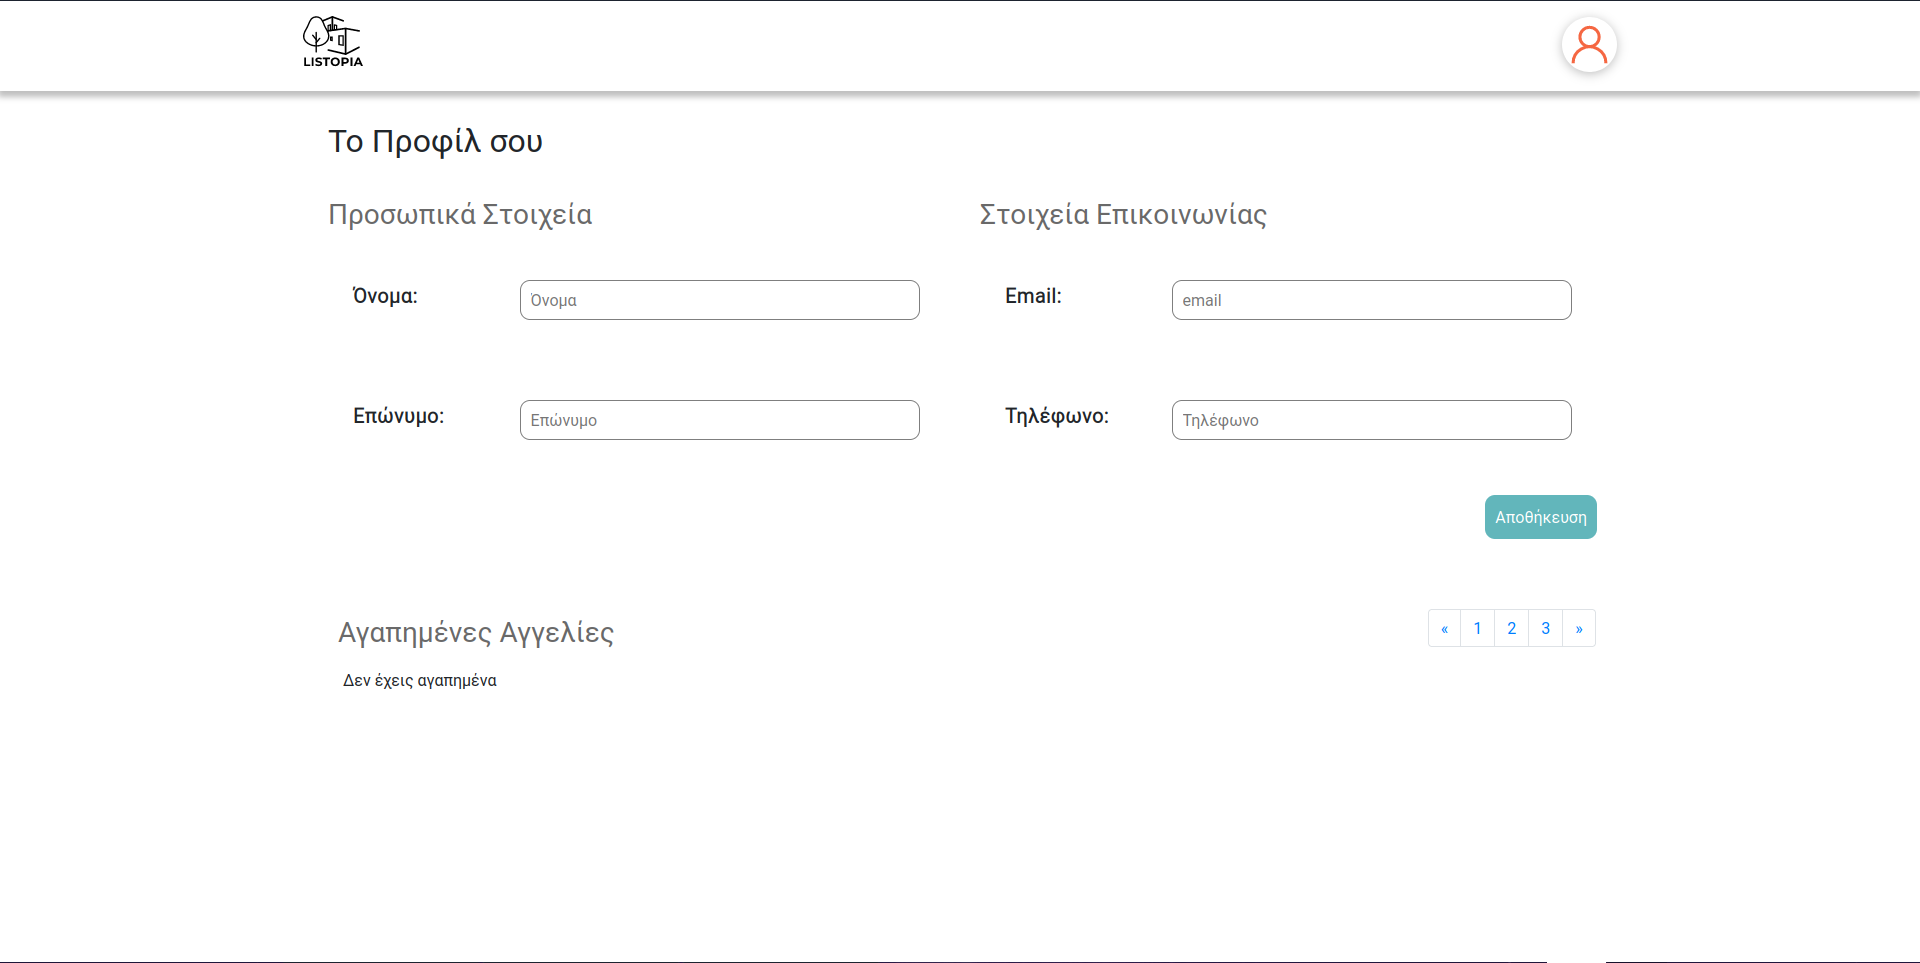
\includegraphics[width=0.8\textwidth]{profile_page.png}
       \caption{Σελίδα Προφίλ Χρήστη}
       \label{fig:control}
\end{figure}

\subsection{Back-end}
\subsection*{Δημιουργία Βάσης Δεδομένων}

\subsection*{Session}

\subsection*{Routes}


\subsection*{Controllers}

\section{Οδηγίεσ χρήσησ και εγκατάστασησ τησ εφαρμογήσ}

\section{Λειτουργία Εφαρμογής}
Η σελίδα μας δύναται να χρησιμοποιηθεί απο οποιονδήποτε απλό χρήστη που επιθυμεί να αναζητήσει διαθέσιμες αγγελίες και να ορίσει τα χαρακτηριστικά που επιθυμεί.

\section{Βιβλιογραφία}
\begin{enumerate}
       \item Υλικό απο το eclass του μαθήματος \href{https://eclass.upatras.gr/courses/EE767/}{Eclass}
       \item \href{https://developer.mozilla.org/en-US/docs/Web/javascript}{JavaScript Docs}
       \item \href{https://developer.mozilla.org/en-US/docs/Learn/Server-side/Express_Nodejs}{Express Docs}
       \item \href{https://www.npmjs.com/}{NPM Docs}
\end{enumerate}

\end{document}